\documentclass{article}

\usepackage{shyne}

% document format
\topmargin 0in
\oddsidemargin 0in
\evensidemargin 0in
\headheight 0in
\headsep 0in
\topskip 0in
\textheight 9in
\textwidth 6.5in
\linespread{1.3}

\begin{document}

\begin{flushleft}
\section*{Group Work - Chapter 10}
\paragraph{1} The file ``Galton-mother-daughter.csv" contains a subset 50 subjects from Galton's mother/daughter height data.
\begin{enumalpha}
\item Create a scatterplot of the data. Does there appear to be a linear relationship between mother's heights and daughter's heights?\\
\medskip
\bt{There does appear to be a linear relationship.}\\
\medskip
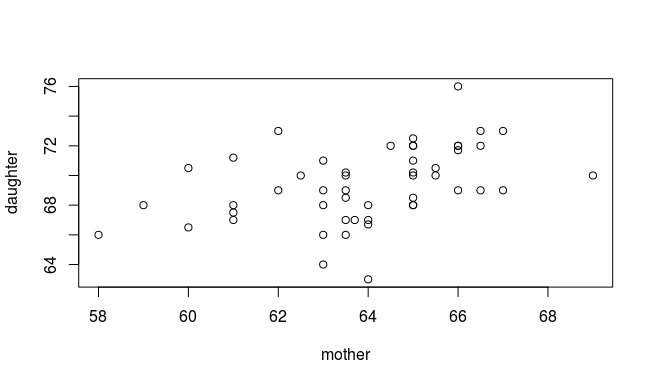
\includegraphics[width=4in]{wk11_mother_daughter}
\vspace{.25in}

\item Conduct a correlation hypothesis test at $\alpha = 0.05$ significance level. If there is significant correlation, how would you describe the strength of the correlation?\\
\medskip
\begin{verbatim}
> cor.test(md$mother, md$daughter)

	Pearson's product-moment correlation

data:  md$mother and md$daughter
t = 3.2743, df = 48, p-value = 0.001969
alternative hypothesis: true correlation is not equal to 0
95 percent confidence interval:
 0.1690464 0.6306322
sample estimates:
      cor 
0.4272886 
\end{verbatim}

$\bv{r = 0.427, \, p = 0.002 < \alpha = 0.05}$. \bt{Reject $\bv{H_0}$. \\ 
There is evidence that heights of mothers and daughters are correlated.\\
Mother and daughter heights are moderately correlated.}

\newpage
\item Find the estimated regression line for the relationship between mother's heights (predictor variable) and daughter's heights (response variable)? Is the slope significantly different than zero?\\
\medskip
\begin{verbatim}
> summary(lm(daughter ~ mother, data=md))

Call:
lm(formula = daughter ~ mother, data = md)

Residuals:
    Min      1Q  Median      3Q     Max 
-6.4070 -1.5703  0.0671  1.5580  5.6189 

Coefficients:
            Estimate Std. Error t value Pr(>|t|)    
(Intercept)  38.2353     9.5144   4.019 0.000206 ***
mother        0.4871     0.1488   3.274 0.001969 ** 
---
Signif. codes:  0 ‘***’ 0.001 ‘**’ 0.01 ‘*’ 0.05 ‘.’ 0.1 ‘ ’ 1

Residual standard error: 2.309 on 48 degrees of freedom
Multiple R-squared:  0.1826,	Adjusted R-squared:  0.1655 
F-statistic: 10.72 on 1 and 48 DF,  p-value: 0.001969
\end{verbatim}

$\bv{\hat y = 38.24 + 0.49 x}$\\
$\bv{t = 3.274, \, p = 0.002}$. \bt{The slope is significantly different than zero.}
\vspace{.5in}

\item What is the best predicted daughter's height for a mother that is 56 inches tall? Is it appropriate to make such a prediction?\\
\medskip
\bt{Since we have a significant correlation, use the regression equation for the prediction.}\\
$\bv{\hat y = 38.24 + 0.49 (56) = 65.68}$\\
\medskip
\begin{verbatim}
> range(md$mother)
[1] 58 69
\end{verbatim}
\bt{Mothers' heights range from 58 to 69 inches. Thus, making a prediction for a mother's height of 56 inches is not appropriate.}


\end{enumalpha}



\newpage
\paragraph{3} The file ``MCA\_scores\_17.csv" on D2L contains average math MCA scores for 11th graders in 2017 by MN public school district, as well as percentage of 11th graders receiving free lunches in the district. Districts with missing data and charter schools are excluded.
\begin{enumalpha}
\item Create a scatterplot of the data. Does there appear to be a linear relationship between percentage of students receiving free lunch and average MCA scores?\\
\medskip
\bt{There does appear to be a linear relationship.}\\
\medskip
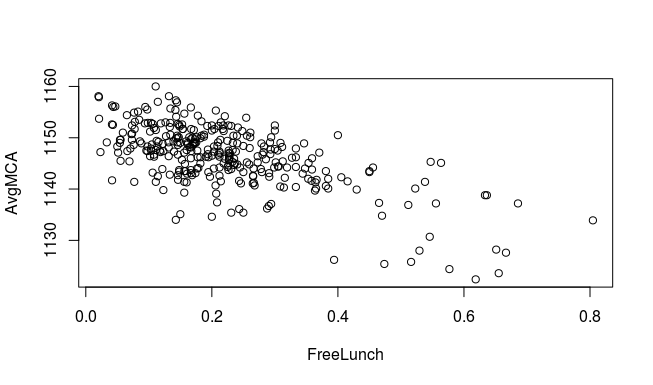
\includegraphics[width=4in]{wk11_mca}
\vspace{.25in}

\item Conduct a correlation hypothesis test at $\alpha = 0.01$ significance level. If there is significant correlation, how would you describe the strength of the correlation?\\
\medskip
\begin{verbatim}
> cor.test(mca$FreeLunch, mca$AvgMCA)

	Pearson's product-moment correlation

data:  mca$FreeLunch and mca$AvgMCA
t = -15.404, df = 321, p-value < 2.2e-16
alternative hypothesis: true correlation is not equal to 0
95 percent confidence interval:
 -0.7105086 -0.5843741
sample estimates:
       cor 
-0.6519282 
\end{verbatim}

$\bv{r = -0.652, \, p  \ll  \alpha = 0.01}$. \bt{Reject $\bv{H_0}$. \\ 
There is evidence that proportion of free lunch students in a district and average MCA scores are correlated.\\
Proportion of free lunch students in a district and average MCA scores are moderately correlated, close to highly correlated.}

\newpage
\item Find the estimated regression line for the relationship between percentage of students receiving free lunch (predictor variable) and average MCA scores (response variable)? Is the slope significantly different than zero?\\
\medskip
\begin{verbatim}
> summary(lm(AvgMCA ~ FreeLunch, data=mca))

Call:
lm(formula = AvgMCA ~ FreeLunch, data = mca)

Residuals:
    Min      1Q  Median      3Q     Max 
-14.984  -2.453   0.359   3.189  10.275 

Coefficients:
             Estimate Std. Error t value Pr(>|t|)    
(Intercept) 1153.0699     0.5042  2286.7   <2e-16 ***
FreeLunch    -30.1726     1.9588   -15.4   <2e-16 ***
---
Signif. codes:  0 ‘***’ 0.001 ‘**’ 0.01 ‘*’ 0.05 ‘.’ 0.1 ‘ ’ 1

Residual standard error: 4.616 on 321 degrees of freedom
Multiple R-squared:  0.425,	Adjusted R-squared:  0.4232 
F-statistic: 237.3 on 1 and 321 DF,  p-value: < 2.2e-16
\end{verbatim}

$\bv{\hat y = 1153.07 - 30.17 x}$\\
$\bv{t = -15.4, \, p \ll 0.0001}$. \bt{The slope is significantly different than zero.}
\vspace{.5in}

\item What is the best predicted average MCA score for a district that has 45\% of 11th grade students receiving free lunch? Is it appropriate to make such a prediction?\\
\medskip
\bt{Since we have a significant correlation, use the regression equation for the prediction.}\\
$\bv{ \hat y = 1153.07 - 30.17 (0.45) = 1139.49}$\\
\medskip
\begin{verbatim}
> range(mca$FreeLunch)
[1] 0.02016129 0.80459770
\end{verbatim}
\bt{Proportions of free lunch students range from 0.0202 to 0.8046. Thus, making a prediction for a free lunch proportion of 0.45 is appropriate.}
\end{enumalpha}


\end{flushleft}
\end{document}